\subsection{Examples}
Users can use \name to create network visualization such as designing network visualization, analyzing networks by layout, exploring large-scale networks, and so on. In this section, we show diverse network visualization examples to illustrate the expressiveness and usability of \name.

\subsubsection{Basic newtrok rendering}
The~\autoref{fig:ex2} shows a Basic network rendering. It can be regard as three parts: initialization, loading data, and rendering. The `testData' illustrates the network data format. In this example, the initialization part hangs the canvas to the document `main'.
\begin{figure}[htbp]
    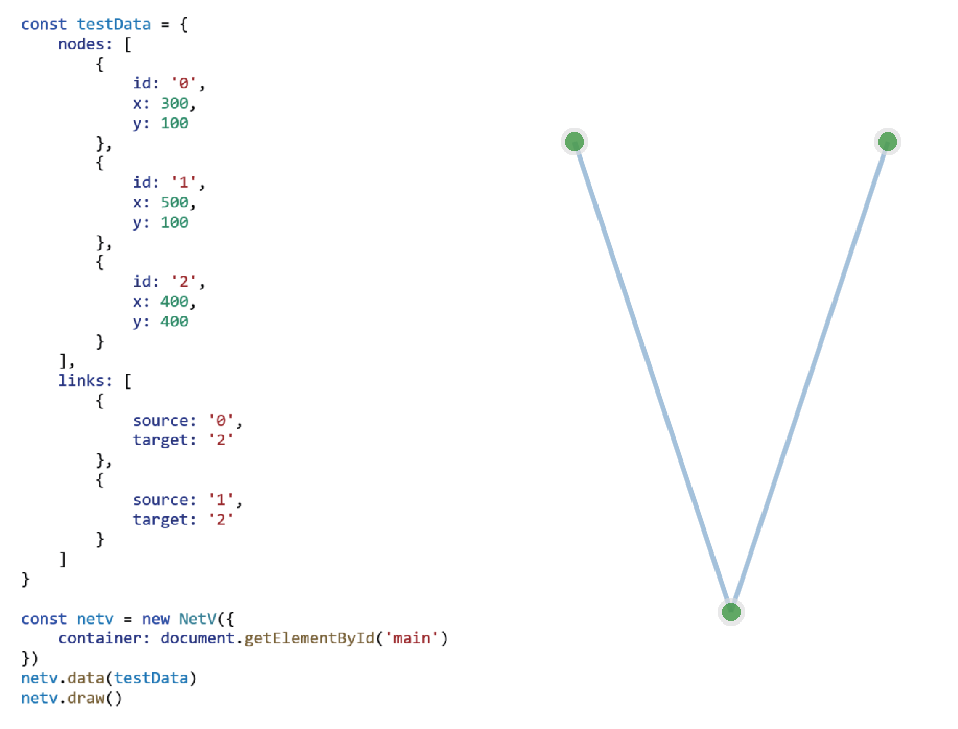
\includegraphics[width=\linewidth]{fig/ex2.eps}
    \caption{
        Basic network rendering.
    }
    \label{fig:ex2}
\end{figure}

\subsubsection{Customized style}
In network visualization, the most important function is to draw a network with different styles, such as color, stroke, radius, and position of elements.
In the~\autoref{fig:ex1}, this example shows the setting of customized style by using \name. Developers can customize the style of each element and set the default style in the initialization part. In particular, initialize configuration items are set in the `configs'.


\begin{figure}[htbp]
    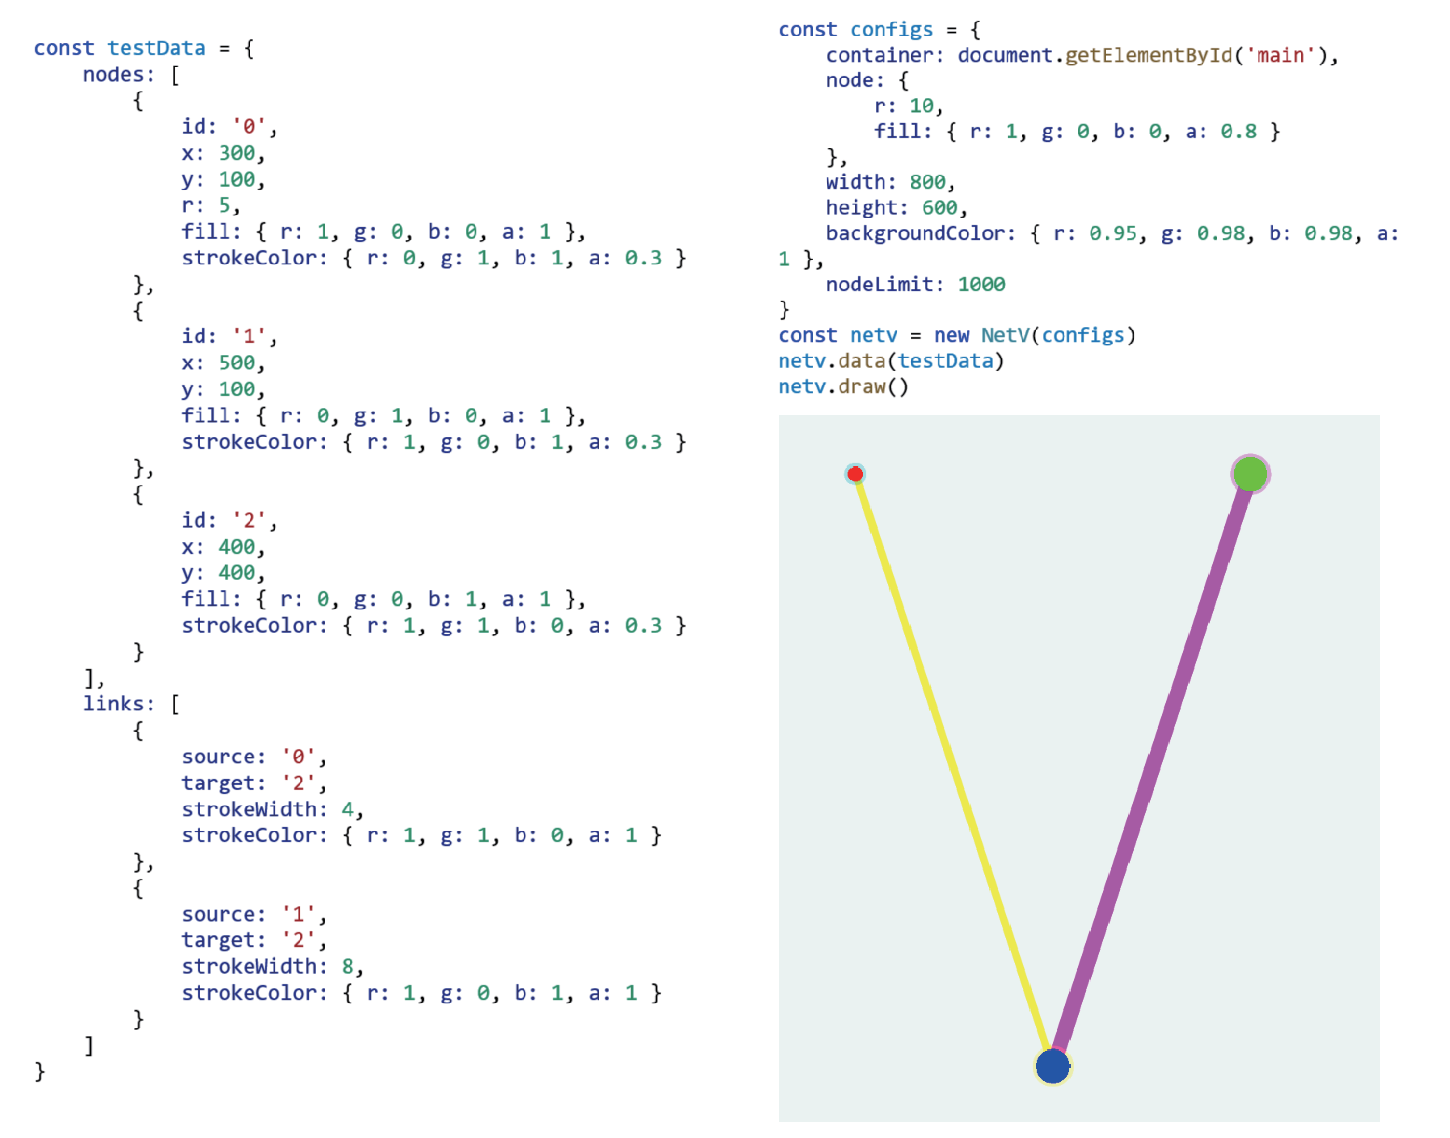
\includegraphics[width=\linewidth]{fig/ex1.eps}
    \caption{
        Customized style.
    }
    \label{fig:ex1}
\end{figure}

\subsubsection{Build-in datasets}
\name supports build-in datasets for users to construct a network visualization (\autoref{fig:ex3}) quickly. The build-in datasets also support the attribute and the position of each node in the network.
Users can the radius and the color of nodes to encode different attributes of nodes.
\begin{figure}[htbp]
    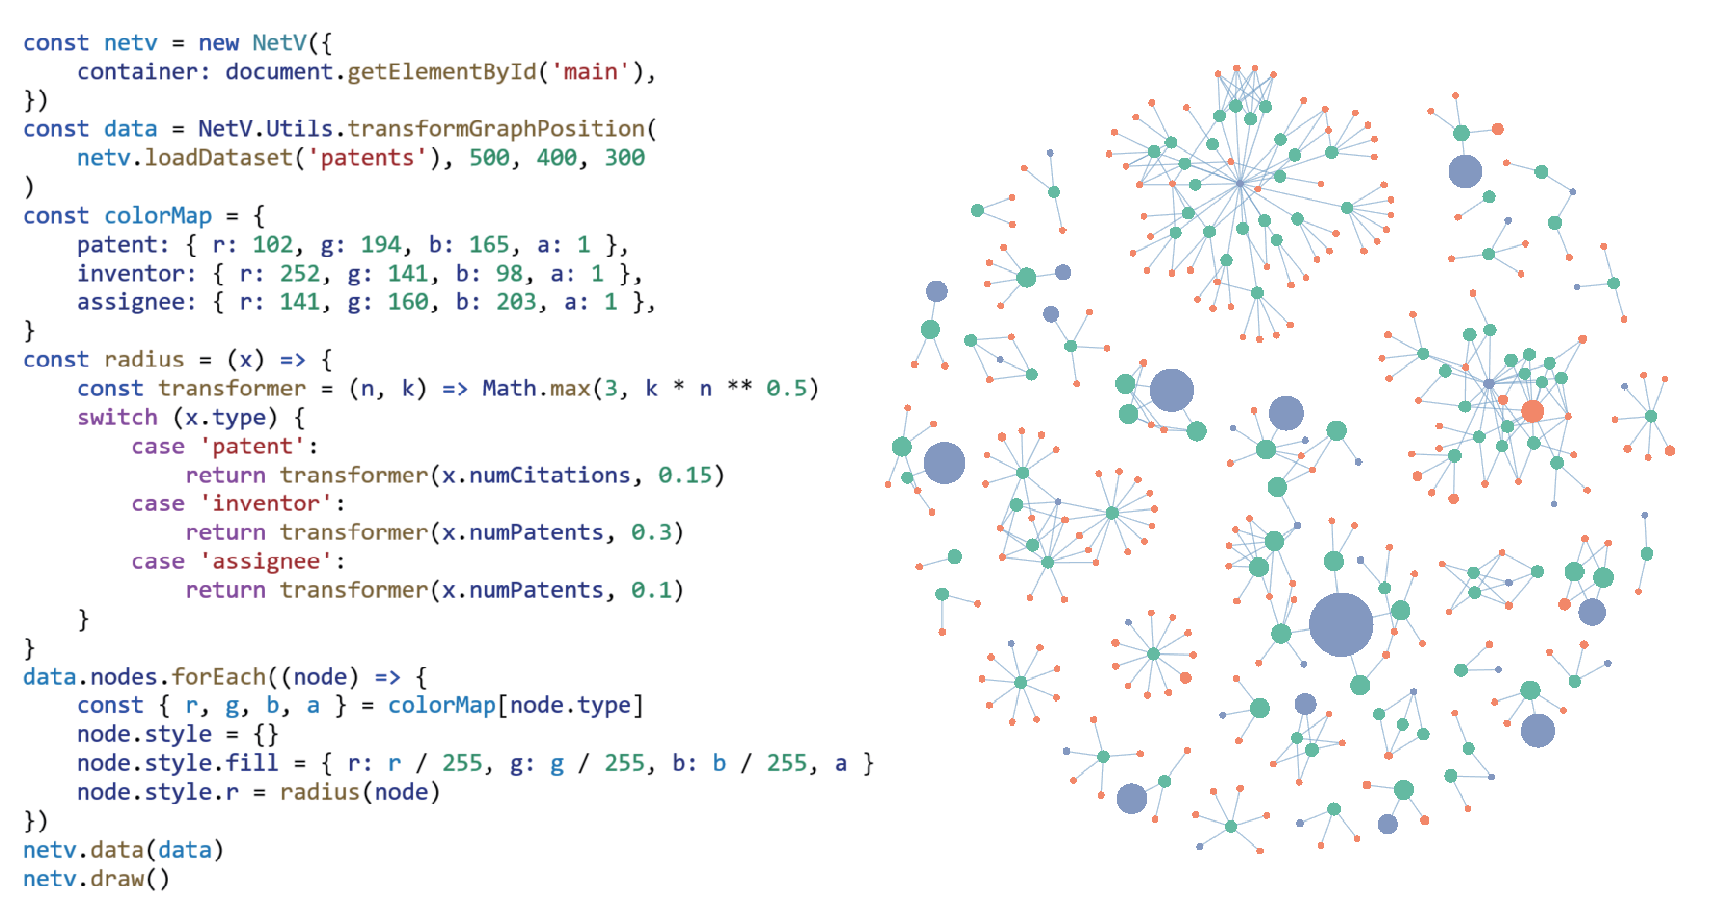
\includegraphics[width=\linewidth]{fig/ex3.eps}
    \caption{
        Build-in datasets.
    }
    \label{fig:ex3}
\end{figure}

\subsubsection{Layout}
\name supports various network layout algorithms. Moreover, developers can implement by combining with external layouts such as D3.js (\autoref{fig:ex4} (a)), or by using \name plugins (\autoref{fig:ex4} (b)). When combining with external layouts, \name acts as a renderer to draw network by layout results.
When using \name layout plugins, it supports developers to controllers of all layout stages.
\begin{figure}[htbp]
    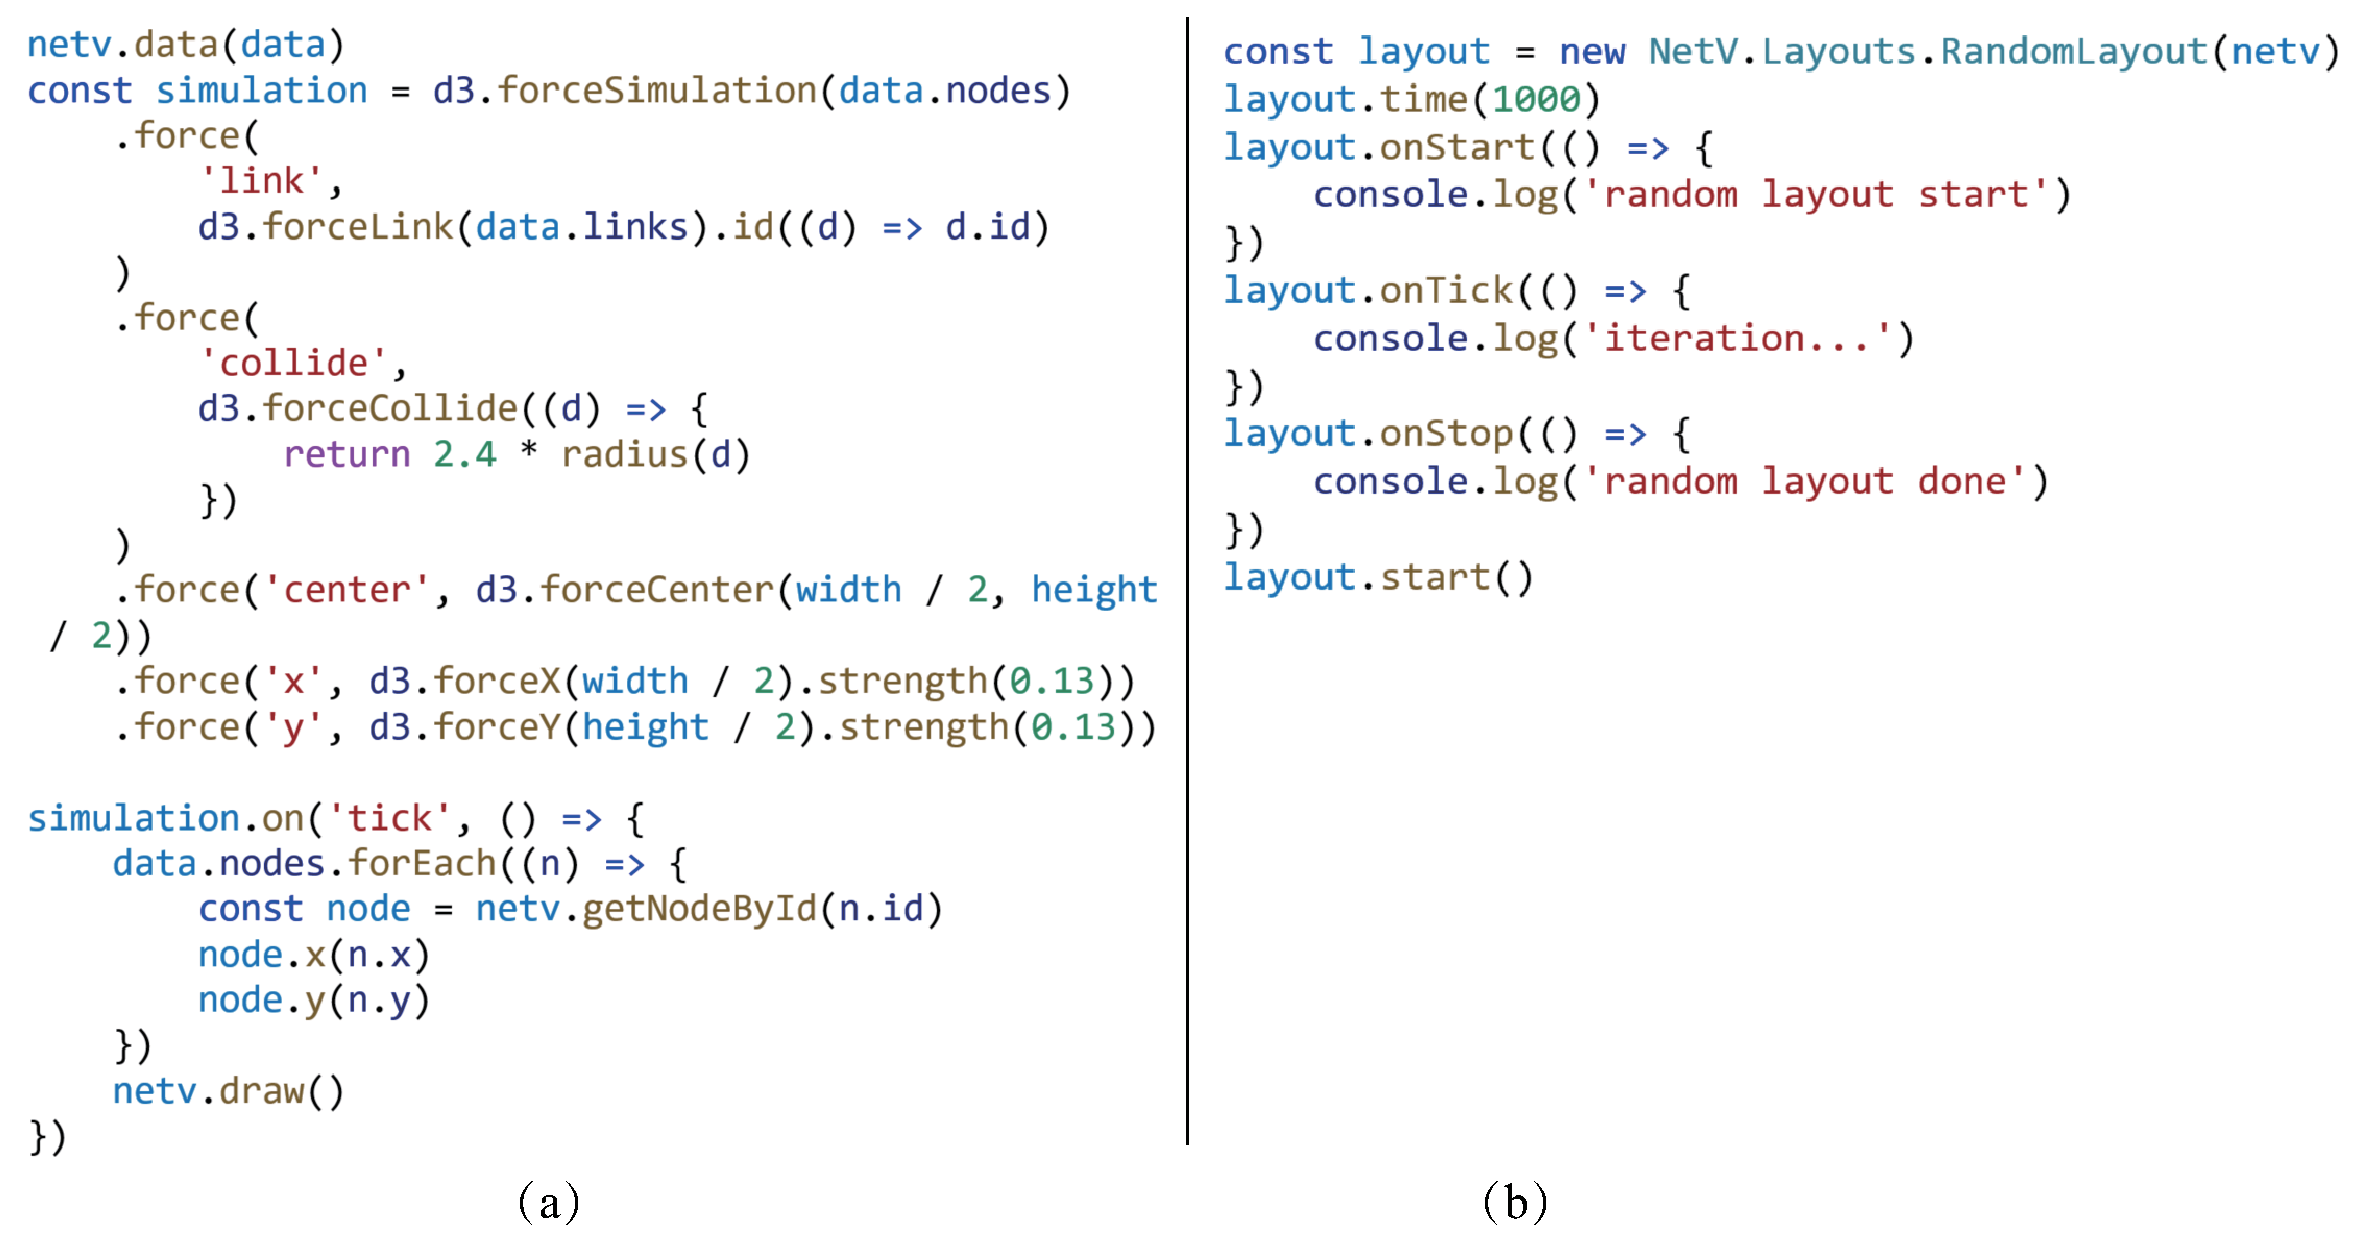
\includegraphics[width=\linewidth]{fig/ex4.eps}
    \caption{
        Layout. (a) Combining with D3.js. (b) Using \name plugins.
    }
    \label{fig:ex4}
\end{figure}

\subsubsection{Large-scale network}
\name aims to render large-scale networks. \autoref{fig:ex5} shows a large-scale network visualization result with 35,590 nodes, and 572,915 links. With the powerful WebGL performance, \name maximum supports for drawing millions of elements.

\begin{figure}[htbp]
    \includegraphics[width=\linewidth]{fig/ex5.eps}
    \caption{
        Large-scale network.
    }
    \label{fig:ex5}
\end{figure}

\subsubsection{Label}
\name supports label rendering with different drawing techniques such as SVG, Canvas, and WebGL. \autoref{fig:ex6} shows the network rendering with labels.

\begin{figure}[htbp]
    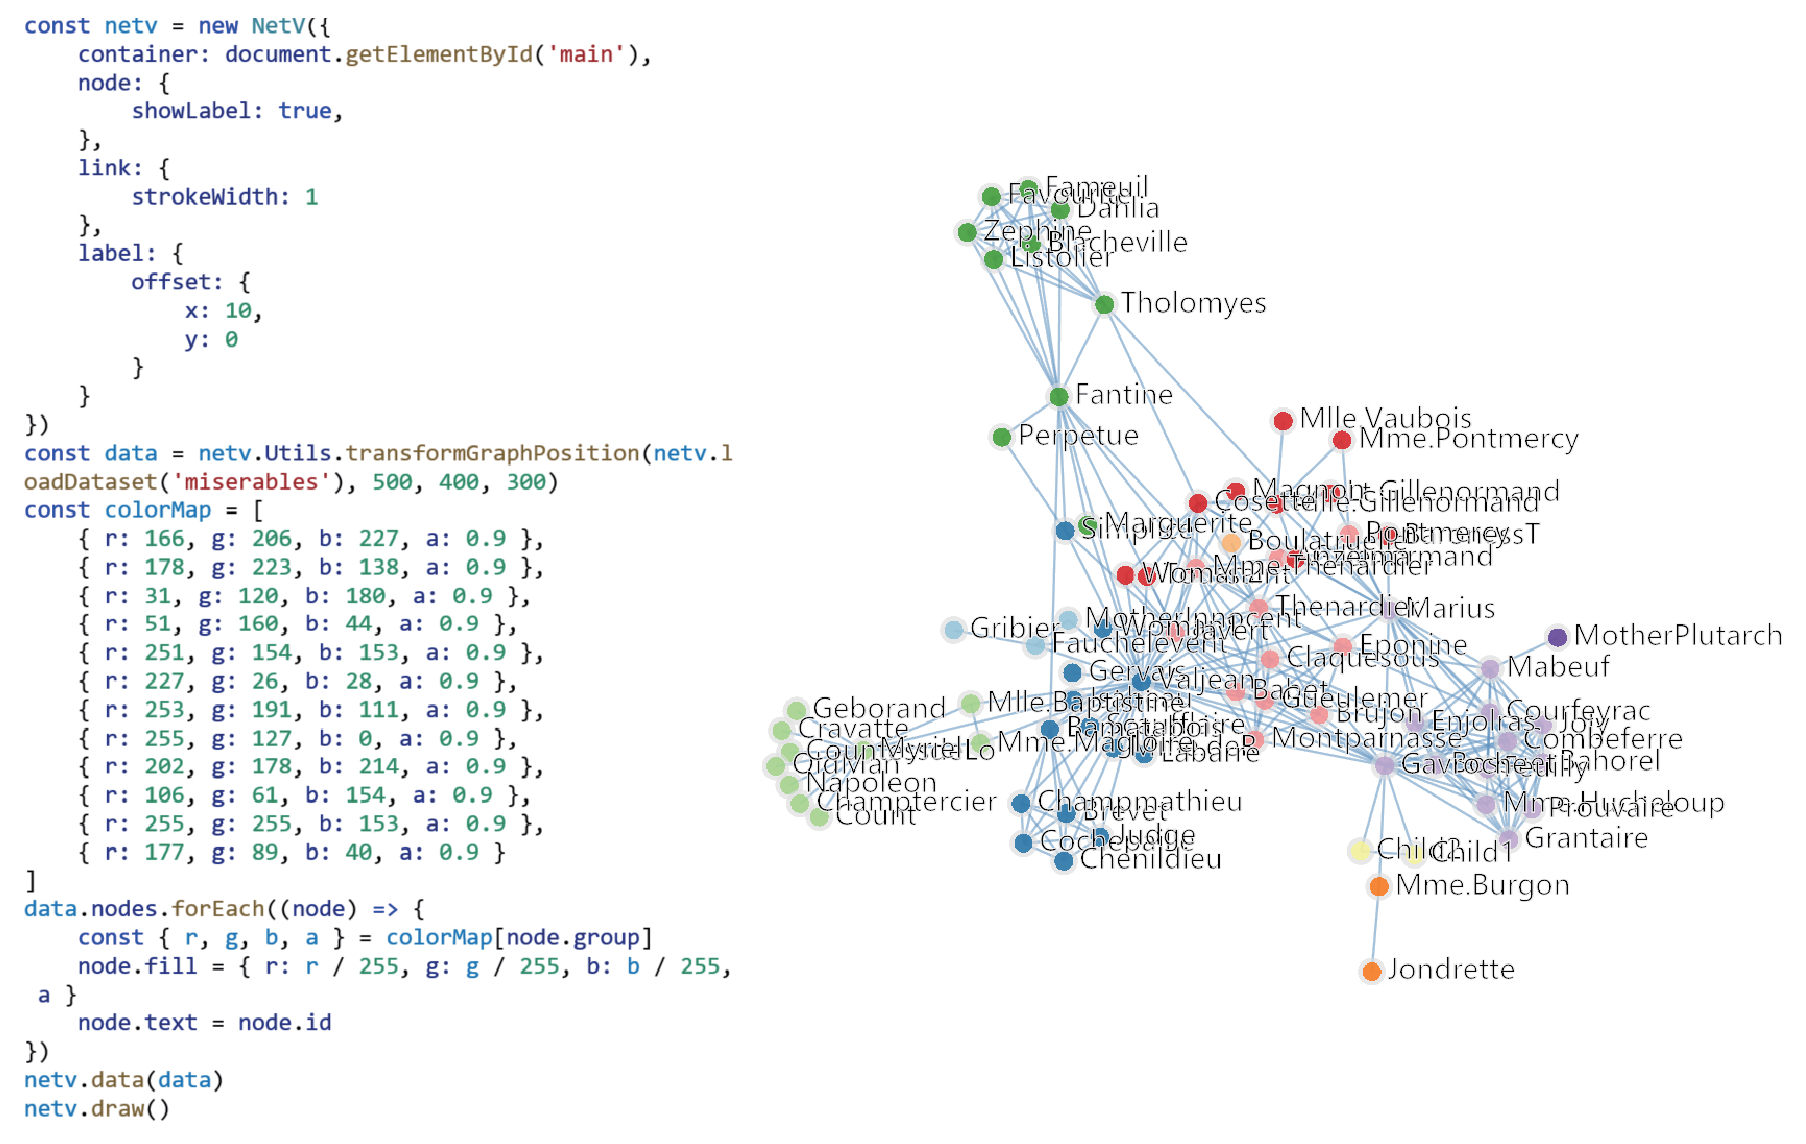
\includegraphics[width=\linewidth]{fig/ex6.eps}
    \caption{
        Label.
    }
    \label{fig:ex6}
\end{figure}